%!TEX root = thesis.tex

\chapter{Visualisation Refinement}
\label{chap:visualisation-refinement}

\section{Rationale}

\section{Design}

\begin{figure}
  \centering 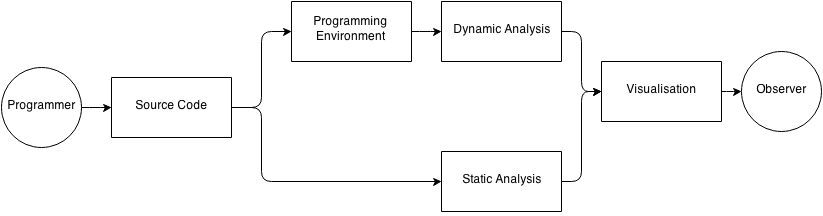
\includegraphics[width=\columnwidth]{../images/diagrams/knowledge-flow}
  \caption{Knowledge flow from programmer to observer as directed by the visualisation technique employed.}
\label{fig:knowledge-flow}
\end{figure}

\begin{figure}
  \centering 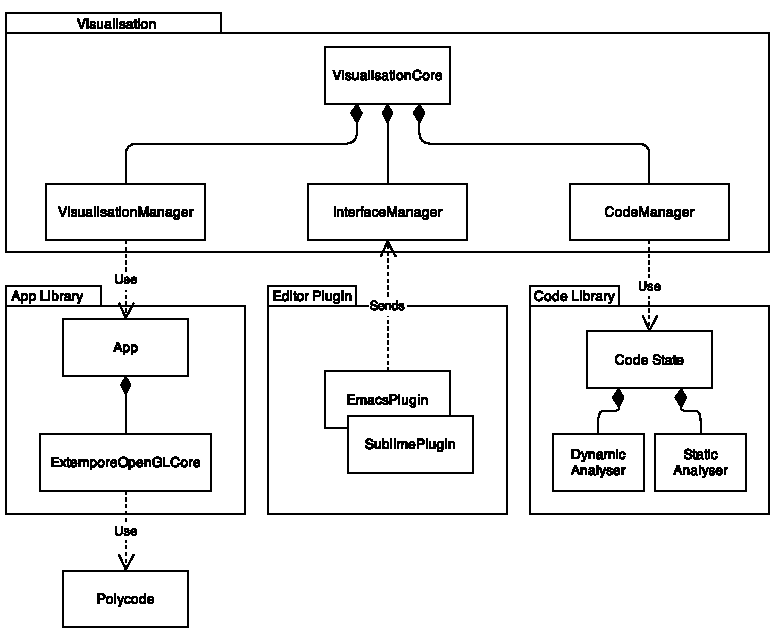
\includegraphics[width=\columnwidth]{../images/diagrams/visualisation-class-diagram}
  \caption{Class diagram of the visualisation technique employed.}
\label{fig:visualisation-class-diagram}
\end{figure}

\section{Analysis}

Both dynamic program analysis and static source code analysis have been used to implement the visualisations (see combined static and dynamic approach taken in \cite{Eisenbarth2003}).

\section{Mappings}